\documentclass[letterpaper,12pt,fleqn]{article}
\usepackage{matharticle}
\usepackage{graphicx}
\pagestyle{plain}
\begin{document}

\begin{center}
\Large Math-19 Homework \#9 Solutions
\end{center}

\vspace{0.5in}

\underline{Problems}

\begin{enumerate}
\item Consider the quadratic function: $y=2-5x-3x^2$.
  \begin{enumerate}
  \item By completing the square, convert the general form to standard form.
    \begin{eqnarray*}
      y &=& 2-5x-3x^2 \\
      &=& -3x^2-5x+2 \\
      &=& -3\left(x^2+\frac{5}{3}x\right)+2 \\
      &=& -3\left(x^2+\frac{5}{3}x+\frac{25}{36}\right)+2+
      3\left(\frac{25}{36}\right) \\
      &=& -3\left(x+\frac{5}{6}\right)^2+2+\frac{25}{12} \\
      y &=& -3\left(x+\frac{5}{6}\right)^2+\frac{49}{12}
    \end{eqnarray*}
    
  \item What are the coordinates of the vertex?

    $\left(-\frac{5}{6},\frac{49}{12}\right)$
    
  \item Is the parabola open up or open down? How do you know?

    Open down because $a=-3<0$.
    
  \item What are the $x$-intercepts (if any)?

    $-3\left(x+\frac{5}{6}\right)^2+\frac{49}{12}=0$ \\
    $3\left(x+\frac{5}{6}\right)^2=\frac{49}{12}$ \\
    $\left(x+\frac{5}{6}\right)^2=\frac{49}{36}$ \\
    $x+\frac{5}{6}=\pm\frac{7}{6}$ \\
    $x=-\frac{5}{6}\pm\frac{7}{6}$ \\
    $x=-2,\frac{1}{3}$

    $(-2,0)$ and $\left(\frac{1}{3},0\right)$
    
  \item What are the $y$-intercepts (if any)?

    $(0,2)$
    
  \item What is the maximum value (if any)?

    This is the $y$-coordinate of the vertex: $\frac{49}{12}$
    
  \item What is the minimum value (if any)?

    none.
    
  \item Where is the axis of symmetry?

    $x=-\frac{5}{6}$
    
  \item Sketch the parabola. All key points must be labeled.

    \begin{tikzpicture}
      \draw (-5,0) -- (5,0);
      \draw (0,-5) -- (0,5);
      \node [draw,circle,fill,scale=0.5] (v) at (-5/6,49/12) {};
      \node [above] at (v) {$\left(-\frac{5}{6},\frac{49}{12}\right)$};
      \node [draw,circle,fill,scale=0.5] (x1) at (-2,0) {};
      \node [below] at (x1) {$(-2,0)$};
      \node [draw,circle,fill,scale=0.5] (x2) at (1/3,0) {};
      \node [below] at (x2) {$\left(\frac{1}{3},0\right)$};
      \draw [dashed] (-5/6,-5) -- (-5/6,5);
      \node [below left] at (-5/6,0) {$-\frac{5}{6}$};
      \draw [smooth,domain=-2.55:0.9] plot ({\x},{2-5*\x-3*\x*\x});
    \end{tikzpicture}
  \end{enumerate}

\item Consider the following polynomial function in factored form:
  \[y=x^2(1-x)^2(2+x)(2-x)^3\]
  \begin{enumerate}
  \item What is the degree?

    First, let's rewrite this with the factors in the proper order:
    \[y=-x^2(x-1)^2(x+2)(x-2)^3\]
    So the leading term is $(x^2)(x^2)(x)(x^3)=x^8$.

    degree$=8$
    
  \item What is the leading term?

    $-x^8$ (see above)

  \item What is the end behavior? How do you know?

    Like $-x^2$ because the power of the leading term (8) is even and the sign
    of the leading coefficient (-1) is $<0$.
    
  \item What are the $x$-intercepts (if any)?

    $(0,0), (1,0), (\pm2,0)$
    
  \item What are the $y$-intercepts (if any)?

    $(0,0)$
    
  \item Sketch the polynomial.

    \begin{tikzpicture}
      \draw (-5,0) -- (5,0);
      \draw (0,-5) -- (0,5);
      \node [draw,circle,fill,scale=0.5] (x1) at (-2,0) {};
      \node [below] at (x1) {$(-2,0)$};
      \node [draw,circle,fill,scale=0.5] (x2) at (0,0) {};
      \node [below] at (x2) {$(0,0)$};
      \node [draw,circle,fill,scale=0.5] (x3) at (1,0) {};
      \node [below] at (x3) {$(1,0)$};
      \node [draw,circle,fill,scale=0.5] (x4) at (2,0) {};
      \node [below] at (x4) {$(2,0)$};
      \draw [smooth] plot coordinates {
        (-2.5,-5) (-2,0) (-1,4) (-0.25,0.25) (0,0)
      };
      \draw [smooth,domain=0:2.45]
      plot ({\x},{(\x)^2*(1-\x)^2*(2+\x)*(2-\x)^3});
    \end{tikzpicture}

    Note the shape at each $x$-intercept.

  \item Attach a screenshot showing the determination of at least one relative
    minimum or maximum.

    Here is the big local maxima (but you can do any of them).

    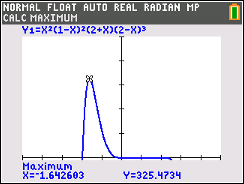
\includegraphics{hw09-2g}
  \end{enumerate}
\end{enumerate}

\end{document}
